%
% File coling2016.tex
%
% Contact: mutiyama@nict.go.jp
%%
%% Based on the style files for COLING-2014, which were, in turn,
%% Based on the style files for ACL-2014, which were, in turn,
%% Based on the style files for ACL-2013, which were, in turn,
%% Based on the style files for ACL-2012, which were, in turn,
%% based on the style files for ACL-2011, which were, in turn, 
%% based on the style files for ACL-2010, which were, in turn, 
%% based on the style files for ACL-IJCNLP-2009, which were, in turn,
%% based on the style files for EACL-2009 and IJCNLP-2008...

%% Based on the style files for EACL 2006 by 
%%e.agirre@ehu.es or Sergi.Balari@uab.es
%% and that of ACL 08 by Joakim Nivre and Noah Smith

\documentclass[11pt]{article}
\usepackage{coling2016}
\usepackage{times}
\usepackage{url}
\usepackage{latexsym}
\usepackage{bm}%used for bm
\usepackage[ruled,vlined,linesnumbered]{algorithm2e}
\usepackage{algorithmic}
\usepackage{amssymb}%used for empty set symbol
\usepackage{amsmath} %used for maths symbols

\usepackage{graphics}
\usepackage{graphicx}
\usepackage{subfigure}
\usepackage{array}
\newcolumntype{L}[1]{>{\raggedright\let\newline\\\arraybackslash\hspace{0pt}}m{#1}}
\newcolumntype{C}[1]{>{\centering\let\newline\\\arraybackslash\hspace{0pt}}m{#1}}
\newcolumntype{R}[1]{>{\raggedleft\let\newline\\\arraybackslash\hspace{0pt}}m{#1}}


%\setlength\titlebox{5cm}

% You can expand the titlebox if you need extra space
% to show all the authors. Please do not make the titlebox
% smaller than 5cm (the original size); we will check this
% in the camera-ready version and ask you to change it back.


\title{Instructions for COLING-2016 Proceedings}

\author{First Author \\
  Affiliation / Address line 1 \\
  Affiliation / Address line 2 \\
  Affiliation / Address line 3 \\
  {\tt email@domain} \\\And
  Second Author \\
  Affiliation / Address line 1 \\
  Affiliation / Address line 2 \\
  Affiliation / Address line 3 \\
  {\tt email@domain} \\}

\date{}

\begin{document}
\maketitle
\begin{abstract}
In the news value theory, the \textit{news unexpectedness} expects the journalists to report the events that are different from the routine things, a.k.a., the normal states. 
For human being, normal states are knowledge learned from news streams and the external environment, and can describe what happened and help to identify what is happening.
In this paper, we propose \textsc{NSDetector}, a high accuracy event detection method that trains normal states better by using knowledge base, which can be treated as the accumulation of happened things. 
In \textsc{NSDetector}, 1) a new data structure \textit{normal states} is proposed to restore what happened; 2) \textit{normal states} can be initialized by knowledge base and further updated by upcoming text streams via our proposed probabilistic model NS-Prior-LDA; 3) events can be detected by normal states with high accuracy.
Experiments on the benchmark \textit{Edinburgh twitter corpus (30 million tweets)} validate the effectiveness of our proposed \textsc{NSDetector}.
\end{abstract}

\section{Introduction}
\label{intro}

With the increasing of cyberspace data, there is a growing need for detecting events accurately. Detecting events can mainly benefit the following three folds: (1) understanding what happened in the corpus without checking every single document manually, and generating the timeline to get a bird's eye view of the corpus\cite{ge2015bring}; (2) being aware what is happening currently, which helps to deal with emergencies\cite{hughes2009twitter}\cite{sakaki2010earthquake}; (3) adding detected events and their types as extra structured data information to organize the unstructured text corpus\cite{ritter2012open}.  

Considering the importance of event detection on the cyberspace data, researchers have have made many efforts, including checking the and the . Therefore, the existing methods are ... and 

In our study, we find out that the key to improve the accuracy of event detection lies in training the normal states of the focused media/site/domain. Based on training normal states accurately, event detection task can be treated as finding terms, articles, or topics which are different from the normal states. 

Our intuition is inspired from the news value theory\cite{galtung1965structure}\cite{caple2013delving}, which emphasizes the \textit{news unexpectedness} -- "the unpredictable or the rare is more newsworthy than the routine"\cite{bell1991language}, and "routine events are difficult to assimilate to the news, which favours the novel, the atypical and the unusual"\cite{montgomery2007discourse}.
Following this guideline, if the journalist knew the normal states, aka, the "routine things" of everyday better, he/she would tend to choose more unexpected news to report. 
We suppose that the ideal event detection system performs like a journalist who can find news from cyberspace with the knowledge of the normal states. 


\section{Related Works}

To train the normal states, the methods of existing systems can be grouped into unsupervised methods and supervised methods based on whether they .

In the first category, the methods treat the normal states as clustered articles\cite{Petrovic:2010uj}\cite{Wurzer:2015wq}, word frequencies\cite{Mathioudakis:2010fc}\cite{Weng:2011wz}, or topics\cite{Diao:2012wj}\cite{Yan:2015wm}. 
Taking the clustering of articles\cite{Petrovic:2010uj}\cite{Wurzer:2015wq} as an example, they model the occurred events as clusters, and link the incoming article with an existing event cluster or assign it as the new detected event.
The decision is based on whether the dissimilarity between the incoming article and existing event clusters is over the user-specified threshold. 

And in the second category, the methods learn the normal states by given the knowledge of \textit{event trigger}\cite{Li2013JointEE}\cite{Nguyen2015EventDA} (usually a single verb or entity mentions). The normal states are trained by the labeled data appeared in a fixed time window.

Both categories of methods have achieved good performance on formal texts, but are hampered by the diverse and rapid changing nature of cyberspace data (e.g., twitter\cite{Asur:2011tc} and reddit\cite{singer2014evolution}).
In the journalist metaphor of news value theory, they have the limited knowledge of normal states (aka "routine things") due to the limited history information used. 
More specifically, 

The second category, train the triggers\cite{Li2013JointEE}\cite{Nguyen2015EventDA}(\textit{But it has some problems here, these methods are used in event extraction, so what's the relationship between event extraction and event detection? and the fired example in \cite{Li2013JointEE}?}). 


Although \cite{Wurzer:2015wq} points out that UMass\cite{Allan:2000wu} and its variants\cite{Petrovic:2010uj}\cite{petrovic2012using}\cite{Wurzer:2015wq} are the state-of-art systems on the Event Detection task for the newswire data, these systems still suffers from the lack of accuracy to applied on more general cyberspace data, such as tweets, emails, and reddit posts. 
The underlying reason is that the normalized Topic Weighted Minimum Cost metric (\(C_{min}\)) used in the Event Detection keep balance between miss and false alarm, which cannot work well on the .
Usually these traditional systems set the ratio of cost between miss alarm and false alarm to 10, preferring recall to precision on detecting events.

Study of event detection on text stream can be divided into three ways: word frequency based, text similarity based and topic model based.

Several word frequency methods have been developed for event detection such as Discrete Fourier Transform\cite{he2007analyzingDFT}, wavelet analysis \cite{weng2011eventWavelet}.
They treat the word's document frequency along timeline as time series and do the analysis in frequency domain. 
DFT method suffers the problem that it can not locate the time point for bursty, while wavelet analysis based method's complexity is very high, which limits its scalability. 

 Text similarity based online event detection methods\cite{petrovic2010streaming}\cite{mccreadie2013scalable}  suffer from the lexical variation which means different words describe the same events.
 Similarity based method can successfully detect the tweet which is retweeted by many times, but fails to find out the event which is described from many different perspectives.
 As a result, many events are duplicately detected due to their popularities, which may bury other events and overwhelm users with duplicated unwanted content.


In contrast, topic model can handle the lexical variation problem with word co-occurrence\cite{blei2003latent}.
%After \cite{blei2006dynamic} and \cite{wang2006topics} introducing time factor into topic model, a number of temporal model has been developed to different tasks.
As many events are highly related to topics, a number of methods based on topic model have been proposed for event detection, including online detection and offline detection.
Lau\cite{lau2012line} introduces an online topic model to track emerging events in microblogs.
It can deal with a massive of tweets, but it doesn't filter out the tweets related to user interests.
Diao\cite{timeUserLDA2012finding}\cite{diao2013unified} show that event detection can benefit from filtering out user interest related tweets. 
And Yan\cite{Yan:2015wm} models the bursty topic by incorporating burstiness of biterms as prior knowledge.
But they are different from ours.
As these models need the whole dataset as the input, they are offline detections, which is not scalability for large dynamic dataset such as microblogs.

\section{Proposed Method}
\subsection{Normal States Initialization}
\subsection{Normal States Maintainence}
\begin{table}
\begin{tabular}{|p{0.1\columnwidth}|p{0.8\columnwidth}|} \hline
\(G^{(0)}\) & Taxonomy's Graph in Knowledge Base\\ \hline
\(G^{(1)}\) & Category-Page Bipartite Graph in Knowledge Base\\ \hline
\(G^{(2)}\) & Page-Content Bipartite Graph in Knowledge Base\\ \hline
\(c\) & topic related category node in \(G^{(0)}\) and \(G^{(1)}\) \\ \hline
\(K_{\bm{KB}}\) & number of pre-defined topics by Knowledge Base \\ \hline
\(f_{c,w}\) & word \(w\)'s normal state (chi-square score) in category \(c\) \\ \hline
\(\lambda\) & normal state weight in  NS-Prior-LDA\\ \hline
\(\tau_{c,w}\) & word \(w\)'s prior knowledge confidence for topic \(c\) in NS-Prior-LDA\\ \hline
\(S_c\) & topic \(c\)'s all normal states related words \\ \hline
\(K\) & number of topics in NS-Prior-LDA such as \(K>K_{\bm{KB}}\)\\ \hline
\(\mathcal{B}_{c, t}\)  & hot words set detected from topic \(k\) at time \(t\)  \\ \hline
\(\mathcal{G}_{c, t}\)  & hot word graph constructed from \(\mathcal{B}_{c, t}\) \\ \hline
\(\mathcal{C}_{c,t,i}\) & event \(i\)-th related words in topic \(c\) at time \(t\) \\ \hline
\(\mathcal{D}_{c,t,i}\) & event \(i\)-th related tweets in topic \(c\) at time \(t\) \\ \hline
\(\rho\) & density threshold for the sub-graph constructed by event words  \\ \hline

\end{tabular}
\label{symbolsInModel}
\end{table}


\begin{algorithm}
\caption{Normal States Initialization from Knowledge Base}
\label{alg:normalStatesInit}

\KwIn{Taxonomy's Graph \(G^{(0)}\), Category-Page Bipartite Graph \(G^{(1)}\), Page-Content Bipartite Graph \(G^{(2)}\), topic related category node \(c\)}
\KwOut{Normal states \(\bm{f}_c\) on topic \(c\)}
\(Pages(c)\leftarrow \varnothing\)\\
DAG \(G^{(0)'} \leftarrow\) Remove Cycles of \(G^{(0)}\) by nodes' HITS-PageRank scores. \\
\(SuccessorNodes(c) \leftarrow \) Breadth-first-traverse(\(G^{(0)},c\))\\
\For{\(node \in SuccessorNodes(c)\)}{
    \(Pages(c) \leftarrow Pages(c) \cup G^{(1)}.neighbours(node)\)\\
}
\(WordFrequencyTable(c) \leftarrow \) do word count on the text contents of \(Pages(c)\) \\
\(WordFrequencyTable(All) \leftarrow \) do word count on the text contents of all pages in \(G^{(2)}\).\\
\For{word \(w\) in WordFrequencyTable(All).keys()}{
    \(\tau_{c,w} \leftarrow \) \(w\)'s chi-square score on \(WordFrequencyTable(c)\) and \(WordFrequencyTable(All)\).
}
\Return{\(\bm{f}_c\)}
\end{algorithm}

\ \ Our theme modeling, want to learn the first \(k\) topics with Wikipedia Article \(k\) topics as close as possible, and we will be Wikipedia article \(k\) before 1000 words) was added to the theme of the word frequency word in the subject a priori distribution on the.
Learning to be the first \(k\) Subject polynomial distribution of the word, referred to as \(\phi_k \), Wikipedia article \(k \) distribution of topics for \(\tau_k \), then this formalized process is expressed as: \(\ \phi_k \sim Dir(\beta + \tau_k) \).
Formal presentation of the explanation is: With prior knowledge \(\tau_k \) after the theme \(\phi_k \) is no longer simply rely on symmetric priori \(\beta \), different words right is not the same weight , such as a discussion of "fashion" theme in Wikipedia, it will refer to "dress", "grand", "blue", "gold" and other words, with the asymmetric priori \(\beta + \tau_k \) after in microblogging "fashion" theme "dress" the proportion will be increased in this way so that microblogging corpus theme tends to Wikipedia topic.
\(\tau_k \) in the first \(v \) words such as formula (\ref{eq: wikiPrior}).
Where \(S_k \) as a set of candidate words: high-quality information to use Wikipedia, we extract the theme \(\phi_k \ \) in the higher-word word frequency candidate set \(S_k \).
We can control set \(S_k \) in size, the size of the control is usually set for 1000.
The number of frequency \(n_{kv} \) for the word \(v \) (\ k) appears in the Wikipedia article themes of: (\ref{wikiPrior eq}).
If the word \(v \) does not appear in the candidate set \(S_k \), and then set a priori knowledge \(\tau_{kv} = 0 \), otherwise, the word frequency is proportional to \(n_{kv} \) with the prior knowledge of weight \(W\).
In the latter experiment, we will be on a priori knowledge of weights \(W \) will be discussed. 

\begin{table}[!htbp]
\begin{tabular}{l}
1. Draw corpus prior distribution \(\bm{m} \sim Dir(\alpha \bm{u})\), where \(\bm{u}\)\\
 \ \ \ \ is the uniform distribution. \\
2. For each topic \(k \in \{1,\cdots,K\}\),\\
\ \ \ \ (a) word distribution on the topic \(\bm{\phi_k} \sim Dir(\bm{\beta}+ \bm{\tau_k})\). \\
    
3. For each document index \(d \in \{1,...,D\}\), \\
\ \ \ \ (a) topic distribution on the document \(\theta_d \sim Dir(\bm{m})\), \\
\ \ \ \ (b) for each word index \(n \in \{1,\cdots,N_d\}\),\\
\ \ \ \ \ \ \ \ i. word's topic assignment \(z_{dn} \sim Multinomial(\theta_d)\), \\
\ \ \ \ \ \ \ \ ii. word \(w_{dn} \sim Multinomial(\phi_{z_{dn}})\). \\
\end{tabular}
\end{table}

\begin{scriptsize}
\begin{equation}
\label{eq:wikiPrior}
\begin{aligned}
\tau_{kv}=
\left\{ \begin{aligned}
\lambda \frac{f_{kv}}{\sum_{v\in S_{kv}}f_{kv}} &,v\in S_{k}\ and  \ k \leq K_{\bm{KB}} \\
0&,v \notin S_{k} \ or \ k > K_{\bm{KB}} \\
\end{aligned}\right.
\end{aligned}
\end{equation}
\end{scriptsize}

\begin{scriptsize}
\begin{equation}
\label{eq:initProbability}
\begin{aligned}
\hat{q}_{k|v}=
\left\{ \begin{aligned}
\frac{\tau_{kv}}{\sum_{k=1}^{K}\tau_{kv}} &,\sum_{k}\tau_{kv}>0 \\
0&, \sum_{k}\tau_{kv}=0 \ and \ k \leq K_{\bm{KB}} \\
1/(K-K_{\bm{KB}})&,\sum_{k}\tau_{kv}=0 \ and \ k > K_{\bm{KB}}
\end{aligned}\right.
\end{aligned}
\end{equation}
\end{scriptsize}

\begin{scriptsize}
\begin{equation}
\label{eq:KBPriorLDAgibbs}
\begin{aligned}
&p(z_{dn}=k|w_{dn}=v,z_{\neg{dn}},w_{\neg{dn}},\alpha\bm{m},\beta,\tau)\\
&\ \ \propto (n^{(d)}_{dk}+\alpha m_k)\frac{n^{(w)}_{kv}+\tau_{kv}+\beta}{n^{(w)}_{k,.}+\tau_{k,.}+V\beta}
\end{aligned}
\end{equation}
\end{scriptsize}

\begin{algorithm}
\caption{NS-Prior-LDA Learning Algorithm}
\label{alg:gibbsSamplingKBPriorLDA}
\KwIn{Documents \(\mathcal{D}\) (a.k.a., \(\bm{w_{1:D}}\)), and normal states \(\bm{f}_{1:K_{\bm{KB}}}\)}
\KwOut{The sufficient statistics \(\bm{n^{(d)}}\), \(\bm{n^{(w)}}\)}
\tcc{Initialization of NS-Prior-LDA}
\For{\(d=1:D\)}{
    \For{\(n=1:N_d\)}{
        \(v=w_{dn}\), sample \(z_{dn}=k\) as Eq(\ref{eq:wikiPrior})(\ref{eq:initProbability}).\\
        Update the sufficient statistics \(n^{(d)}_{d,k}\), \(n^{(w)}_{k,v}\).\\
            }
        }
\For{\(i= 1:I\)}{
    \tcc{E-Step of NS-Prior-LDA}
    \For{\(i=1:I_E\)}{
        \For{\(d=1:D\)}{
            \For{\(n=1:N_d\)}{
                Set \(v=w_{dn}\), and reset the sufficient statistics \(n^{(d)}_{d,z_{dn}}\), \(n^{(w)}_{z_{dn},v}\).\\
                Resample \(z_{dn}=k\) as Eq(\ref{eq:wikiPrior})(\ref{eq:KBPriorLDAgibbs}).\\
                Update the sufficient statistics \(n^{(d)}_{d,k}\), \(n^{(w)}_{k,v}\).\\
            }
        }
    }
    \tcc{M-Step of NS-Prior-LDA}
    Optimize \(\alpha \bm{m}\) by the fixed-point iteration\cite{wallach2008structured}. 
}
\Return{\(\bm{n^{(w)}}\)}
\end{algorithm}

\subsection{Detecting Events from Normal States}
The state of attention of social issue k at time t in cyberspace is binary, namely at the peak or not at the peak. We denote it by hidden binary variable \(s_{k,t}\), which is 1 or 0. We do the inference for the hidden variable \(s_{k,t}\) according to Poisson distribution according to Reference\cite{Diao:2012wj} 10,11. If the state of attention of social issue k at time t is "not at peak", then the probability density function is 
\(p(x_{k,t}|s_{k,t}=0)=e^{-\mu_0 }  \frac{\mu_0^{x_{k,t}}}{x_{k,t}!}\) otherwise the probability density function is \(p(x_{k,t}|s_{k,t}=0)=e^{-\mu_1 }  \frac{\mu_1^{x_{k,t}}}{x_{k,t}!}\)
In the above functions the symbol \(x_{k,t}\) denotes the attention of social issue \(k\) at time \(t\) , the symbol A denotes the constant, \(\mu_0\) and \(\mu_1\) represent the average of \(x_{k,t}\) at peak and not at peak respectively. The state \(s_{k,t}\) is inferred from \(ratio=\frac{p(x_{k,t} |s_{k,t}=0)}{p(x_{k,t} |s_{k,t}=1)} \).
In calculation, we use the log ratio to determine whether the attention is at peak as in equation (\ref{eq:logratio}). \(\log ratio>0 \) indicates that the attention of social issue \(k\) at time \(t\) is not at peak, otherwise at peak. 
\begin{equation}
\label{eq:logratio}
\log ratio=-(\mu_0-\mu_1 )+x_{k,t}(\log \mu_0 -\log⁡ \mu_1)
\end{equation}

\begin{algorithm}
\label{alg:eventKeywordsSearchMethod}
\caption{Spectral Clustering Based Event Phrase Extraction}
\label{alg:eventKeywordsSearchMethod}
\KwIn{\(\mathcal{B}_{k,t},\mathcal{G}_{k,t},\rho\)}
\KwOut{\(\mathcal{C}_{k,t}\)}
\(n_{k,t}\)=number of connected component in \(\mathcal{G}_{k,t}\)\\
\For{\(n \in \{ n_{k,t}, \cdots, |\mathcal{G}_{k,t}|\}\) }{
    \(\mathcal{C}_{k,t}=SpectralClustering(\mathcal{G}_{k,t},n)\)\\
    \If{\(min_{i\in \{1,\cdots,n\}} Density(\mathcal{C}_{k,t,i},\mathcal{G}_{k,t})>\rho\)}{
        return \(\mathcal{C}_{k,t}\)
    }
}
\end{algorithm}


\textbf{event} phrase Mining
% Refer to bursty.py
\ \ Microblogging mining events can be represented by a variety of ways, a single word, phrase, or topic.
Here we use the form of phrase, said event.
In this paper, the phrase indicates that the event is due to the fact that: the same period of time when there are multiple areas of internal hot words appear, a collection of hot words \(\mathcal{B}_{k, t} \) between the hot words great probability is interrelated. For example, observed "mac", "os", "lion" three words are in a state of emergency.
In fact, the state of emergency three words is to publish a new system "mac os lion" event caused by Apple, in order to find the association between words and events, we use spectral clustering based search methods.

As shown in Figure \ref{fig: windowsBurstyWordGraph} below, we will one area, a hot word of the time window and hot words between to diagram.
Hot words set \(\mathcal{B}_{k, t} \) formed in FIG using \textbf{hot word graph} \(\mathcal{G}_{k, t} = (\mathcal{B}_{k, t}, \mathcal{E}_{k, t}) \) indicates,
\(\mathcal{E}_{k, t} = \{(a, b) | a \in \mathcal{B}_{k, t}, b \in \mathcal{B}_{k, t }, PMI (\mathcal{D}_{k, t}, a, b)> 0 \} \), where \(PMI (\mathcal{D}_{k, t}, a, b) \) the field \(k \) time window \(t \) related microblog \(\mathcal{D}_{k, t} \) on the word \(a\) and the word \(b\) point metric information between each other.
% Refer to bursty.py getSimGraph () function

Given a field \(k\) and the time window \(t\), in which the number of events can not be determined in advance.
The two most extreme situations are: events coarse granularity, said the event is equal to the number of Figure \(\mathcal{G}_{k, t} \) in the number of connected components; events finer granularity display, event number equal to \(\mathcal{G}_{k, t} \) the number of points.
To do this, we use the Density to the degree of density of quantum graphs \(2 \#Edge / (\# Node \ cdot (\# Node-1)) \), the more the greater if the edge density in the range of Density in \((0,1] \).
Density can be a good indicator to determine the size indicates the event: too many unrelated phrases to put together an event can not be represented, too fine particle size, such as a single word can represent only part of the event; only in close co-occurrence of the phrase to a reasonable It indicates that the event granularity.
To this end, we have designed events phrase search algorithm \ref{alg:eventKeywordsSearchMethod}: We try to find a reasonable number of spectral clustering Clustering \(n \), let \(n \) from a smaller value ( event corresponds to coarser granularity representation) to start the search, then the most likely cluster cluster size is too large, its performance is the clustering results in one or more small Density indicators; continue to increase the number of clusters \(n \), the event represents reduced size, reduced the size of clusters of clusters, thus making the Density index increases; when all cluster clustering Density indicators are larger than the threshold \(\tau \), the search terminates, returning clustering results \(\mathcal{C}_{k, t}\).
As the above process algorithm \ref{alg:eventKeywordsSearchMethod} description line 2 to line 5, we use in practice \(\rho = 0.6 \).
We call \(\mathcal{C}_{k, t} \) results in each cluster to cluster \textbf{event} phrase.

\section{Experiments}
\subsection{Effects of Normal States Initialization}
We use 20newsgroups\cite{lang1995newsweeder} dataset\footnote{http://qwone.com/~jason/20Newsgroups} to check the effects of normal states initialization.


What's NPMI? maybe can refer to \cite{Aletras2013EvaluatingTC}\cite{Rder2015ExploringTS}\footnote{https://github.com/AKSW/Palmetto}.
\begin{table}[]
\centering
\caption{My caption}
\label{my-label}
\begin{tabular}{|l|l|}
\hline
comp.graphics            & Category:Computer graphics      \\ \hline
comp.os.ms-windows.misc  & Category:Microsoft Windows      \\ \hline
comp.sys.ibm.pc.hardware & Category:IBM personal computers \\ \hline
comp.sys.mac.hardware    & Category:Macintosh computers    \\ \hline
comp.windows.x           & Category:X Window System        \\ \hline
rec.autos                & Category:Automobiles            \\ \hline
rec.motorcycles          & Category:Motorcycles            \\ \hline
rec.sport.baseball       & Category:Baseball               \\ \hline
rec.sport.hockey         & Category:Hockey                 \\ \hline
sci.crypt                & Category:Cryptography           \\ \hline
sci.electronics          & Category:Electronics            \\ \hline
sci.med                  & Category:Medicine               \\ \hline
sci.space                & Category:Outer space            \\ \hline
misc.forsale             & Category:Sales                  \\ \hline
talk.politics.misc       & Category:Politics               \\ \hline
talk.politics.guns       & Category:Gun politics          \\ \hline
talk.politics.mideast    & Category:Middle East           \\ \hline
talk.religion.misc       & Category:Religion               \\ \hline
alt.atheism              & Category:Atheism                \\ \hline
soc.religion.christian   & Category:Christians             \\ \hline
\end{tabular}
\end{table}


\begin{figure}
        \centering
        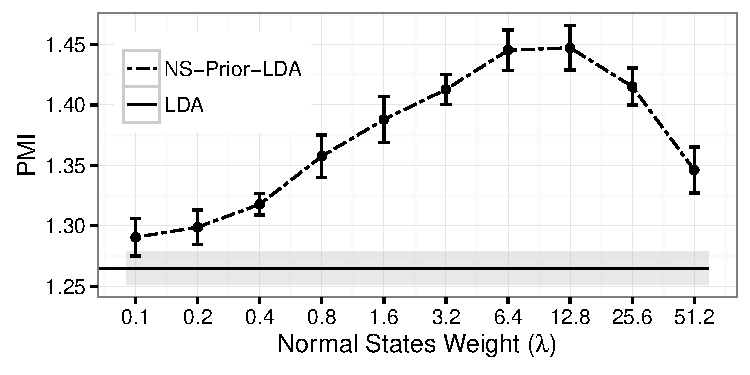
\includegraphics[height=4.0cm]{img/pmi.pdf}
        \caption{The quality of all twitter topics learned by NS-Prior-LDA increases with normal states weight (\(\lambda\)) before \(\lambda=12.8\). The optimized PMI is gained with moderate normal states weight when considering topics \(k\leq K_{\bm{KB}}\) and topics \(k > K_{\bm{KB}}\) together.}
\end{figure}

\begin{figure}
        \centering
        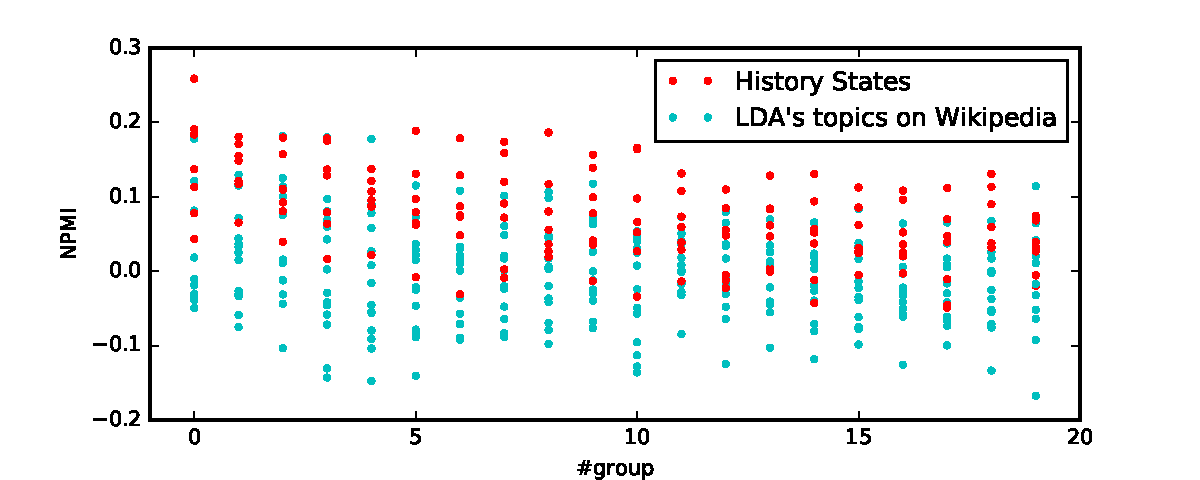
\includegraphics[width=1.0\columnwidth]{img/NPMI.pdf}
        \caption{NPMI}
\end{figure}



\begin{table}
\centering
\caption{The PMI of twitter topics learned by NS-Prior-LDA, its variant, and other baselines}
    \begin{tabular}{|l|l|c|}
    \hline
    Model & Prior Knowledge & PMI \\ \hline
    LDA & None  & 1.265 \(\pm\) 0.013     \\ \hline
    BBTM\cite{Yan:2015wm} & None    & 1.467 \(\pm\) 0.017     \\ \hline
    NS-Prior-LDA\(^{(-)}\)   &   \begin{tabular}[c]{@{}l@{}}\footnotesize{Words in categories simply}\\ \footnotesize{extracted from Wikipedia}\end{tabular} & 1.439 \(\pm\) 0.010     \\ \hline
    NS-Prior-LDA         & \begin{tabular}[c]{@{}l@{}}\footnotesize{Normal states initialized} \\\footnotesize{from wikipedia}\end{tabular} & 1.523 \(\pm\) 0.017     \\ \hline
    \end{tabular}
\label{tbl:NS-Prior-LDA}
\end{table}

\begin{table*}[ht]
\centering
\caption{My caption}
\label{my-label}
\scalebox{0.88}{
\begin{tabular}{|cc|cc|cc|cc|cc|cc|}
\hline
\multicolumn{2}{|c|}{\textit{Aviation}} & \multicolumn{2}{c|}{\textit{Health}} & \multicolumn{2}{c|}{\textit{Middle East}} & \multicolumn{2}{c|}{\textit{Military}} & \multicolumn{2}{c|}{\textit{Mobile Phones}} & \multicolumn{2}{c|}{\textit{Video Games}} \\
\begin{tabular}[c]{@{}c@{}}Normal\\ States\end{tabular} & \begin{tabular}[c]{@{}c@{}}Topical\\ Words\end{tabular} & \begin{tabular}[c]{@{}c@{}}Normal\\ States\end{tabular} & \begin{tabular}[c]{@{}c@{}}Topical\\ Words\end{tabular} & \begin{tabular}[c]{@{}c@{}}Normal\\ States\end{tabular} & \begin{tabular}[c]{@{}c@{}}Topical\\ Words\end{tabular} & \begin{tabular}[c]{@{}c@{}}Normal\\ States\end{tabular} & \begin{tabular}[c]{@{}c@{}}Topical\\ Words\end{tabular} & \begin{tabular}[c]{@{}c@{}}Normal\\ States\end{tabular} & \begin{tabular}[c]{@{}c@{}}Topical\\ Words\end{tabular} & \begin{tabular}[c]{@{}c@{}}Normal\\ States\end{tabular} & \begin{tabular}[c]{@{}c@{}}Topical\\ Words\end{tabular} \\ 
\hline
aircraft & air\scriptsize(3253) & health & weight\scriptsize(16344) & al & \textcolor{red}{\textit{\#syria}}\scriptsize(4212) & army & killed\scriptsize(4055)  & android & iphone\scriptsize (13674) & game & games\scriptsize(8812) \\ 
air & plane & patients & loss & israel & \textcolor{red}{\textit{\#bahrain}} & military & news & mobile & apple & player & liked \\ 
airport & flight & medical & diet & iran & people & air & \textcolor{red}{\textit{\#libya}}\scriptsize(3503) & nokia & android & playstation & free \\ 
flight & time & disease & health & arab & israel & command & libya & ios & app & gameplay & xbox \\
airline & airlines & treatment & cancer & israeli & police & force & rebels & phone & ipad & nintendo & 360 \\
airlines & news & hospital & lose & egypt & \textcolor{red}{\textit{\#libya}}\scriptsize(2557) & regiment & people & samsung & samsung & games & playing \\
aviation & boat & patient & fat & egyptian & \#egypt & forces & police & game & mobile & players & played \\
flying & airport & clinical & tips & ibn & news & squadron & war & app & blackberry & xbox &iphone\scriptsize(2820)\\
pilot & force & symptoms & treatment & jerusalem & \#israel & infantry & libyan & iphone & tablet & mode & time\\
squadron & fly & cancer & body & syria & world & battle & attack & htc & apps & arcade & \textcolor{red}{\textit{ps3}}\\
flights & hurricane & cells & healthy & iraq & syria & commander & u.s. & smartphone & free & wii & trailer\\
pilots & navy & blood & study & palestinian & protest & ship & gaddafi & phones & \#android & multiplayer & online\\
raf & flying & therapy & pain & syrian & israeli & corps & army & blackberry & htc & sega & hours\\
airways & aircraft & drug & exercise & iranian & egypt & navy & forces & apps & google & console & ipad\\
fighter & \textcolor{red}{\textit{irene}} & medicine & \#health & ottoman & al & brigade & pakistan & ipad & galaxy & enemies & app\\
boeing & crew & brain & natural & islamic & syrian & battalion & afghanistan & gsm & ios & characters & player\\
runway & sky & care & disease & iraqi & protesters & lieutenant & military & lte & store & playable & wii\\
force & crash & syndrome & acne & abu & arab & aircraft & attacks & symbian & windows & character & ops\\
crashed & jet & infection & hair & jewish & rights & officer & troops & devices & mac & video & download\\
flew & pilot & disorder & surgery & persian & libya & naval & dead & smartphones & phones & graphics & nintendo\\
\hline
\end{tabular}
}
\end{table*}

\begin{table*}[ht]
\centering
\caption{My caption}
\label{my-label}
\subtable[Twitter Dataset Statistics]{
\begin{tabular}{|l|r|}
\hline
Time range & \begin{tabular}[c]{@{}l@{}}2011/06/30\\ -2011/09/15\end{tabular} \\ \hline
Tweet Number & 36,627,434 \\ \hline
\begin{tabular}[c]{@{}l@{}}Event Number \\ in Benchmark1\end{tabular} & 27 \\ \hline
\begin{tabular}[c]{@{}l@{}}Event Number \\ in Benchmark2\end{tabular} & 523 \\ \hline
\end{tabular}
}\quad \quad
\subtable[Event Detection Results]{
    \begin{tabular}{|l|l|l|l|l|}
    \hline
    Method & \begin{tabular}[c]{@{}l@{}}Recall@ \\ Benchmark1\end{tabular} & \begin{tabular}[c]{@{}l@{}}Precision@ \\ Benchmark2\end{tabular} & \begin{tabular}[c]{@{}l@{}}Recall@ \\ Benchmark2\end{tabular} & \begin{tabular}[c]{@{}l@{}}DERate(Duplicate \\ Event Rate)\end{tabular} \\ \hline
    UMass System & 0.882 & 0.138 & 0.941 & 0.071 \\ \hline
    LSH & 0.824 & 0.095 & 0.803 & 0.302 \\ \hline
    TimeUserLDA & 0.353 & 0.536 & 0.071 & 0.054 \\ \hline
    Twevent & 0.824 & 0.697 & 0.641 & 0.113 \\ \hline
    EDCoW & 0.412 & 0.756 & 0.119 & 0.290 \\ \hline
    BBTM & 0.647 & 0.809 & 0.170 & 0.045 \\ \hline
    \textsc{NSDetector} & 1.000 & 0.894 & 0.950 & 0.042 \\ \hline
    \end{tabular}
}
\end{table*}

\begin{table*}[ht]
\centering
\caption{Events about \textit{vehicles} detected by systems between 2011-07-20 and 2011-07-30}
\label{my-label}
\begin{tabular}{|l|L{3cm}|l|c|}
\hline
\multicolumn{1}{|c|}{Date} & \multicolumn{1}{c|}{Event key words} & \multicolumn{1}{c|}{Representative event tweet} & \multicolumn{1}{c|}{\begin{tabular}[c]{@{}c@{}}Number of \\ event tweet\end{tabular}} \\ \hline
7/20/11 & \begin{tabular}[c]{@{}l@{}}American, airlines, \\ order, planes\end{tabular} & \begin{tabular}[c]{@{}l@{}}NDTV: American Airlines orders 460 new planes from \\ Boeing, Airbus http://bit.ly/p1ZgYG\end{tabular} & 31 \\ \hline
7/26/11 & \begin{tabular}[c]{@{}l@{}}Morocco, military, \\ plane, crash\end{tabular} & \begin{tabular}[c]{@{}l@{}}BBC News - Morocco military plane crash kills 78 \\ http://t.co/uwnLv8L\end{tabular} & 36 \\ \hline
7/27/11 & air, Canada & \begin{tabular}[c]{@{}l@{}}Smoke in galley forces Air Canada flight back to airport. \\ Plane landed safely in Sydney, Australia after dumping fuel\end{tabular} & 48 \\ \hline
7/30/11 & \begin{tabular}[c]{@{}l@{}}Caribbean, airlines, \\ crashes, Guyana\end{tabular} & \begin{tabular}[c]{@{}l@{}}Caribbean Airlines Jet Crash-Lands In Guyana All 163 \\ Passengers, Crew Survive http://t.co/qPVD3WJ\end{tabular} & 57 \\ \hline
\end{tabular}
\end{table*}

\begin{table*}[ht]
\centering
\caption{Events about \textit{military} detected by systems between 2011-07-20 and 2011-07-30}
\label{my-label}
\begin{tabular}{|l|L{3cm}|l|l|}
\hline
Date & Event key words & Representative event tweet & \begin{tabular}[c]{@{}l@{}}Number of \\ event tweet\end{tabular} \\ \hline
7/20/11 & \begin{tabular}[c]{@{}l@{}}Serbia, crimes, \\ fugitive, arrests\end{tabular} & Serbia: Serbia arrests last war crimes fugitive-TV- Reuters & 27 \\ \hline
7/20/11 & Somalia, famine & \begin{tabular}[c]{@{}l@{}}UN declares famine in Somalia. What can we do to save \\ 3.7million lives? http://bit.ly/r1Rq7R\end{tabular} & 89 \\ \hline
7/21/11 & \begin{tabular}[c]{@{}l@{}}U.S., military, \\accept, gay, \\lesbian, openly\end{tabular} & \begin{tabular}[c]{@{}l@{}}RT @cnnbrk: Pentagon is set to certify that the U.S. military \\ is prepared to accept openly gay and lesbian service members \\ \#dadt\end{tabular} & 20 \\ \hline
7/22/11 & \begin{tabular}[c]{@{}l@{}}Norway, Oslo,\\ attacks, bombing\end{tabular} & \begin{tabular}[c]{@{}l@{}}Terror Attacks Devastate Norway: A bomb ripped through \\ government offices in Oslo and a gunman...˙http://dlvr.it/cLbk8\end{tabular} & 557 \\ \hline
7/23/11 & Gunman, rink & \begin{tabular}[c]{@{}l@{}}Gunman Kills Self, 5 Others at Texas Roller Rink \\ http://dlvr.it/cLcTH\end{tabular} & 43 \\ \hline
7/26/11 & \begin{tabular}[c]{@{}l@{}}Kandahar, mayor, \\ suicide, attack\end{tabular} & \begin{tabular}[c]{@{}l@{}}TELEGRAPH{]}: Kandahar mayor killed by Afghan suicide \\ bomber: The mayor of Kandahar, the biggest city in south \_\end{tabular} & 25 \\ \hline
7/28/11 & Ft., Hood, attack & Possible Ft. Hood Attack Thwarted http://t.co/BSJ33hk & 20 \\ \hline
7/28/11 & \begin{tabular}[c]{@{}l@{}}Libyan, rebel, \\ gunned\end{tabular} & \begin{tabular}[c]{@{}l@{}}Libyan rebel chief gunned down in Benghazi \\ http://sns.mx/prfvy1\end{tabular} & 44 \\ \hline
\end{tabular}
\end{table*}

\begin{figure*}
    \label{fig:algorithm}
    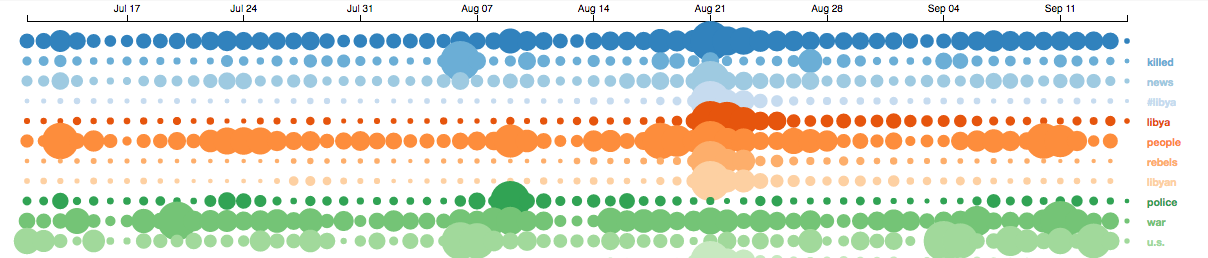
\includegraphics[width=1.0\textwidth]{img/screenShot.png}
    \caption{An illustration of the time series of Military related states on Twitter dataset from 2011-06-30 to 2011-09-15.}
\end{figure*}

\subsection{Data set and experiment settings}
\textbf{Data set.} We conduct the empirical analysis on a twitter dataset which is constructed by \cite{petrovic2012using} and widely used by previous event detection researches \cite{petrovic2013can} \cite{Wurzer:2015wq}. 
Due to the developer policy of Twitter\footnote{https://dev.twitter.com/overview/terms/policy}, \cite{petrovic2012using} only redistributes tweets' IDs\footnote{http://demeter.inf.ed.ac.uk/cross/docs/fsd\_corpus.tar.gz}.
We collected the tweets' contents according to the IDs with the help of Twitter API. 

%TODO
The benchmark \textit{Edinburgh twitter corpus} contains 27 manually labeled events\cite{petrovic2013can}\footnote{\url{http://demeter.inf.ed.ac.uk/cross/docs/Newswire_Events.tar.gz}} and 90 million tweets. Though we cannot get the whole dataset due to the limit of Twitter API, after neccessary pre-processing, our rebuilt dataset still contains 36,627,434 tweets, which spans identically from 2011/06/30 to 2011/09/15, and also covers 27 labeled events.
More details of the original dataset are described in \cite{petrovic2010edinburgh}.

20-newsgroup\footnote{http://qwone.com/~jason/20Newsgroups/}

\textbf{Benchmark1} The first set of the ground truth about events in the corpus are provided by \cite{petrovic2013can}, which is mentioned above. 
And 27 events ...

\textbf{Benchmark2} here.

\textbf{Normal States Initialization} here.

\textbf{Baseline}

UMass System

LSH

TimeUserLDA

Twevent

EDCoW

BBTM

\textbf{Model Setting}

\subsection{Validity of Normal States}
\textbf{Topic Coherence} \cite{roder2015exploring}
\subsection{Topical Words Learned by NS-Prior-LDA}
\textbf{PMI}
\subsection{Evaluation of Detected Events}
\textbf{Precision} Precision@Benchmark1, Precision@Benchmark2

\textbf{Recall}

\textbf{Accuracy}

\textbf{DERate(Duplicate Event Rate)}
\subsection{Case Study}


\subsection{Application on Reddit}

\section{Conclusions \& Future Work}
Microbiolog is mixed with user interests and external events.
The quality of event detection in microblog depends on how we distinguish them.
We exploit user profile to discover events by filtering out user interest-related tweets.
We further treat the arriving data as stream and run the detection in online learning style.
The experiments demonstrates that our method is effective and efficient for online event detection in microblogs.
\bibliographystyle{coling2016}
\bibliography{paperbib}


\end{document}
